\documentclass[11pt]{article}
\usepackage[margin=1in]{geometry}
\usepackage{amsmath,amssymb,mathtools}
\usepackage{microtype}
\usepackage{hyperref}
\hypersetup{colorlinks=true, linkcolor=blue, citecolor=blue, urlcolor=blue}
\usepackage{tikz}
\usetikzlibrary{arrows.meta,positioning}

\newcommand{\E}{\mathbb{E}}
\newcommand{\KL}{\mathrm{KL}}
\newcommand{\Hent}{\mathrm{H}}

\title{An Imbalanced-Tree Toy Example for KL- and Entropy-Regularized Fine-Tuning}
\author{}
\date{\today}

\begin{document}
\maketitle

\paragraph{Objective and closed form}
Let $\mathcal{Y}$ be a finite set, $\pi_{\mathrm{pre}}$ a pretrained distribution on $\mathcal{Y}$, and $r:\mathcal{Y}\to\mathbb{R}$ a reward. For $\alpha>0$ and $\mu\ge 0$, consider
\begin{equation}\label{eq:objective}
J_\mu(\pi)
:= \E_{\pi}[r(Y)]
   + \mu\,\Hent(\pi)
   - \alpha\,\KL\!\big(\pi \,\|\, \pi_{\mathrm{pre}}\big),
\qquad
\Hent(\pi)=-\sum_{y}\pi(y)\log \pi(y).
\end{equation}
Maximizing \eqref{eq:objective} over all distributions $\pi$ on $\mathcal{Y}$ admits the closed-form solution
\begin{equation}\label{eq:pi_star}
\pi^*_\mu(y)
:= \frac{1}{Z}\,
\exp\!\Big(\frac{r(y)}{\mu+\alpha}\Big)\,
\pi_{\mathrm{pre}}(y)^{\frac{\alpha}{\mu+\alpha}},
\qquad
Z=\sum_{u\in\mathcal{Y}}
\exp\!\Big(\frac{r(u)}{\mu+\alpha}\Big)\,
\pi_{\mathrm{pre}}(u)^{\frac{\alpha}{\mu+\alpha}}.
\end{equation}
Assume $Z\in(0,\infty)$.
When $\mu=0$ this reduces to the classical entropy-regularized fine-tuning tilt
$\pi^*_0(y)\propto \exp\big(r(y)/\alpha\big)\,\pi_{\mathrm{pre}}(y)$.

\paragraph{Imbalanced depth-2 tree (pen-and-paper example)}
Consider a depth-2 tree with leaves $\mathcal{Y}=\{L1,L2,R1\}$.
At the root:
left with probability $0.99$, right with probability $0.01$.
From the left branch: choose between $L1$ and $L2$ with conditional probability $1/2$ each.
From the right branch: a single leaf $R1$.
Thus the pretrained distribution over leaves is
\[
\pi_{\mathrm{pre}}(L1)=\pi_{\mathrm{pre}}(L2)=0.99\times\tfrac{1}{2}=0.495,
\qquad
\pi_{\mathrm{pre}}(R1)=0.01.
\]
Assign rewards
\[
r(L1)=1,\qquad r(R1)=1,\qquad r(L2)=0,
\]
so there are two equal reward maxima ($L1$ and $R1$), one at the end of each main branch.

\medskip
\noindent
For ease of visualization, Figure~\ref{fig:tree} sketches the tree and annotates probabilities and rewards.

\begin{figure}[h]
\centering
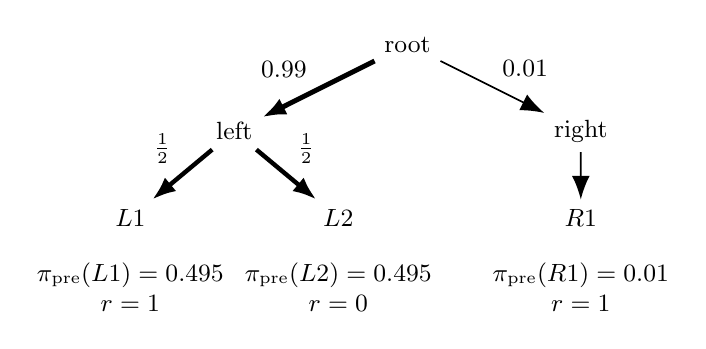
\begin{tikzpicture}[scale=1.1, every node/.style={font=\small}]
  % Nodes
  \node (root) at (0,0) {$\text{root}$};
  \node (left)  at (-2,-1) {left};
  \node (right) at ( 2,-1) {right};
  \node (L1)    at (-3.2,-2) {$L1$};
  \node (L2)    at (-0.8,-2) {$L2$};
  \node (R1)    at ( 2.0,-2) {$R1$};

  % Edges with thickness reflecting prior
  \draw[line width=1.8pt,-{Latex[length=3mm]}] (root) -- node[above left] {$0.99$} (left);
  \draw[line width=0.6pt,-{Latex[length=3mm]}] (root) -- node[above right] {$0.01$} (right);
  \draw[line width=1.6pt,-{Latex[length=3mm]}] (left) -- node[above left] {$\tfrac{1}{2}$} (L1);
  \draw[line width=1.6pt,-{Latex[length=3mm]}] (left) -- node[above right] {$\tfrac{1}{2}$} (L2);
  \draw[line width=0.6pt,-{Latex[length=3mm]}] (right) -- (R1);

  % Annotations
  \node[below=6pt of L1, align=center] {$\pi_{\mathrm{pre}}(L1)=0.495$\\$r=1$};
  \node[below=6pt of L2, align=center] {$\pi_{\mathrm{pre}}(L2)=0.495$\\$r=0$};
  \node[below=6pt of R1, align=center] {$\pi_{\mathrm{pre}}(R1)=0.01$\\$r=1$};
\end{tikzpicture}
\caption{Imbalanced depth-2 tree: two equal reward maxima ($L1$ and $R1$) but a highly skewed pretrained prior toward the left branch.}
\label{fig:tree}
\end{figure}

\paragraph{Classical case ($\mu=0$): collapse down the fat branch for small $\alpha$}
From \eqref{eq:pi_star} with $\mu=0$,
\[
\pi^*_0(y)\propto e^{r(y)/\alpha}\,\pi_{\mathrm{pre}}(y).
\]
Within the set of reward maximizers $\{L1,R1\}$,
\[
\frac{\pi^*_0(L1)}{\pi^*_0(R1)}=
\frac{e^{1/\alpha}\cdot 0.495}{e^{1/\alpha}\cdot 0.01}=\frac{0.495}{0.01}\approx 49.5.
\]
As $\alpha\downarrow 0$, the factor $e^{1/\alpha}$ overwhelms $L2$ ($r=0$), so all mass concentrates on the maximizer set $\{L1,R1\}$. Within $\{L1,R1\}$, the ratio $49.5$ is independent of $\alpha$; hence the limit distribution is the prior-restricted normalization:
\[
\pi^*_0(L1)=\frac{0.495}{0.495+0.01}\approx 0.9802,\qquad
\pi^*_0(R1)=\frac{0.01}{0.495+0.01}\approx 0.0198.
\]
Thus, for $\mu=0$, the optimizer does not rebalance equal-reward modes; it inherits the pretrained skew toward the left branch.

\medskip
\noindent\textbf{Explicit normalization for $\mu=0$.}
Define unnormalized scores $s(y)=e^{r(y)/\alpha}\,\pi_{\mathrm{pre}}(y)$. In the tree,
\[
s(L1)=e^{1/\alpha}\cdot 0.495,\qquad s(R1)=e^{1/\alpha}\cdot 0.01,\qquad s(L2)=0.495,
\]
and the normalizer is
\[
Z=s(L1)+s(R1)+s(L2)=0.495 + (0.495+0.01)e^{1/\alpha}=0.495+0.505\,e^{1/\alpha}.
\]
Therefore
\[
\pi^*_0(L1)=\frac{e^{1/\alpha}\cdot 0.495}{0.495+0.505\,e^{1/\alpha}},\quad
\pi^*_0(R1)=\frac{e^{1/\alpha}\cdot 0.01}{0.495+0.505\,e^{1/\alpha}},\quad
\pi^*_0(L2)=\frac{0.495}{0.495+0.505\,e^{1/\alpha}}.
\]
Dividing numerator and denominator by $e^{1/\alpha}$ gives the limits as $\alpha\downarrow 0$:
\[
\pi^*_0(L1)\to \frac{0.495}{0.505}\approx 0.9802,\qquad
\pi^*_0(R1)\to \frac{0.01}{0.505}\approx 0.0198,\qquad
\pi^*_0(L2)\to 0.
\]
In particular,
\[
\pi^*_0(L2)=\frac{0.495}{0.495+0.505\,e^{1/\alpha}}
=\frac{1}{1+\frac{0.505}{0.495}\,e^{1/\alpha}} \xrightarrow[\alpha\downarrow 0]{} 0,
\]
which makes precise the statement that the factor $e^{1/\alpha}$ overwhelms the $r=0$ leaf.

\paragraph{New objective ($\mu>0$): symmetric coverage of reward modes}
From \eqref{eq:pi_star}, for general $\mu>0$,
\[
\pi^*_\mu(y)\propto
\exp\!\Big(\frac{r(y)}{\mu+\alpha}\Big)\,
\pi_{\mathrm{pre}}(y)^{\frac{\alpha}{\mu+\alpha}}.
\]
For the two equal-reward leaves, the relative weight is
\begin{equation}\label{eq:ratio}
\frac{\pi^*_\mu(L1)}{\pi^*_\mu(R1)}
= \left(\frac{\pi_{\mathrm{pre}}(L1)}{\pi_{\mathrm{pre}}(R1)}\right)^{\!\frac{\alpha}{\mu+\alpha}}
\exp\!\Big(\frac{r(L1)-r(R1)}{\mu+\alpha}\Big)
= 49.5^{\frac{\alpha}{\mu+\alpha}}.
\end{equation}
Thus:
\begin{itemize}
  \item If $\mu=0$, \eqref{eq:ratio} equals $49.5$, reproducing collapse.
  \item If $\mu>0$ is fixed and $\alpha\downarrow 0$, then $\alpha/(\mu+\alpha)\to 0$ and \eqref{eq:ratio}$\to 1$:
        the two reward maxima receive \emph{equal} mass, independent of the prior skew.
\end{itemize}
Moreover, relative to $L2$,
\[
\frac{\pi^*_\mu(L2)}{\pi^*_\mu(L1)}=
\exp\!\Big(\!-\frac{1}{\mu+\alpha}\Big),
\]
so the degree of separation between reward-$1$ and reward-$0$ leaves is governed by the ``temperature'' $\mu+\alpha$.

\paragraph{Concrete numbers}
Take $\alpha=0.05$.
\begin{itemize}
  \item $\mu=0$:
        $\pi^*_0(L1):\pi^*_0(R1)=49.5:1$ among the two maxima,
        and $L2$ is negligible compared to $e^{1/\alpha}=e^{20}$.
        Normalizing over all three leaves yields approximately
        $\pi^*_0(L1)\approx 0.98$, $\pi^*_0(R1)\approx 0.02$, $\pi^*_0(L2)\approx 0$.
  \item $\mu=1$:
        here $\mu+\alpha=1.05$ and $\alpha/(\mu+\alpha)\approx 0.0476$,
        so $\pi^*_\mu(L1)/\pi^*_\mu(R1)\approx 49.5^{0.0476}\approx 1.20$,
        and $\pi^*_\mu(L1)/\pi^*_\mu(L2)\approx e^{1/1.05}\approx 2.59$.
        Normalizing gives roughly
        $\pi^*_\mu(L1)\approx 0.45$, $\pi^*_\mu(R1)\approx 0.38$, $\pi^*_\mu(L2)\approx 0.17$:
        both high-reward leaves are well represented.
\end{itemize}

\paragraph{Takeaway}
In an imbalanced tree, the classical objective ($\mu=0$) favors high-reward leaves along high-prior branches and can \emph{collapse} onto a single subtree when $\alpha$ is small.
Adding an explicit entropy term $\mu \Hent(\pi)$ (with $\mu>0$) reduces the exponent on the prior factor to $\alpha/(\mu+\alpha)$ and raises the effective temperature to $\mu+\alpha$:
this neutralizes prior-induced asymmetries among equal reward maxima and yields broader, multi-modal coverage aligned with the true data distribution $q$ when it is multi-modal.

\paragraph{Optional derivation (Lagrangian, discrete)}
Expanding $J_\mu(\pi)$ and introducing a multiplier $\lambda$ for $\sum_y \pi(y)=1$ yields the stationarity condition
\[
r(y) - (\mu+\alpha)\big(\log \pi(y)+1\big) + \alpha\log \pi_{\mathrm{pre}}(y) + \lambda = 0
\quad (\text{for } \pi(y)>0),
\]
which rearranges to $\log \pi(y)=\tfrac{1}{\mu+\alpha}\big(r(y)+\alpha\log \pi_{\mathrm{pre}}(y)\big) - \log Z$, giving \eqref{eq:pi_star}.
Strict concavity for $\mu+\alpha>0$ implies uniqueness.

\end{document}


